% VoiceGuard — final project paper (Applicative Learning Project, Woxsen University).
% Build:  cd docs/paper && tectonic voiceguard.tex
% Figures come from `python src/make_figures.py`; every number in this paper is
% produced by the scripts in src/ (see Appendix A).
\documentclass[11pt,a4paper]{article}

\usepackage[margin=2.5cm,headheight=28pt]{geometry}
\usepackage[T1]{fontenc}
\usepackage{lmodern}
\usepackage{microtype}
\usepackage{amsmath}
\usepackage{graphicx}
\usepackage{booktabs}
\usepackage{tabularx}
\usepackage{array}
\usepackage{xcolor}
\usepackage{enumitem}
\usepackage{fancyhdr}
\usepackage{caption}
\usepackage{tikz}
\usetikzlibrary{positioning,arrows.meta,shapes.misc}
\usepackage[hidelinks]{hyperref}

\definecolor{wxred}{HTML}{E8384F}
\definecolor{ink2}{HTML}{444B55}
\captionsetup{font=small,labelfont=bf}
\setlist{itemsep=2pt,topsep=4pt}

\newcommand{\logo}[1]{\IfFileExists{figures/woxsen-logo.png}{
\includegraphics[height=#1]{figures/woxsen-logo.png}}{{\sffamily\bfseries\color{wxred}WOXSEN}\,{\sffamily\small UNIVERSITY}}}

\pagestyle{fancy}
\fancyhf{}
\fancyhead[L]{\logo{22pt}}
\fancyhead[R]{\small VoiceGuard: Prosodic Fingerprinting for Voice-Clone Detection}
\fancyfoot[C]{\thepage}
\renewcommand{\headrulewidth}{0.5pt}

\begin{document}

% ---------------------------------------------------------------- title page
\begin{titlepage}
\centering
\vspace*{1cm}
\logo{2.6cm}\par
\vspace{1.6cm}
{\Huge VOICEGUARD\par}
\vspace{0.4cm}
{\Large\itshape Detecting AI-Generated Voice Clones via Prosodic Irregularity Fingerprinting\par}
\vspace{1.4cm}
{\Large\bfseries Applicative Learning Project: Final Report\par}
\vspace{0.8cm}
{\large Submitted by\par}
\vspace{0.4cm}
\begin{tabular}{rl}
\textbf{Name} & \textbf{Roll No.}\\
Shreya Mary Kurien & 24WU0102014\\
Krishiv Saluja & 24WU0102025\\
Raghav Parashar & 24WU0102104\\
Taha Pathan & 24WU0102190\\
Thrinath M & 24WU0102202\\
\end{tabular}
\par\vspace{1.4cm}
{\bfseries Department of Artificial Intelligence and Machine Learning\\School of Technology, Woxsen University\par}
\vspace{1cm}
{\bfseries Under the Guidance of: Prof.\ Monday Jubrin Abdullahi\par}
\vfill
{\large October 2026\par}
\end{titlepage}

\tableofcontents
\clearpage

% ---------------------------------------------------------------- abstract
\section*{Abstract}
\addcontentsline{toc}{section}{Abstract}
Zero-shot voice cloners can reproduce a person's voice from seconds of audio, and most deepfake-audio detectors chase spectral artifacts that each new generator removes. VoiceGuard tests a behavioural alternative: prosodic fingerprinting, the habitual timing, melody, loudness dynamics and pausing of an individual speaker. We enroll three speakers from 20 read sentences each, describe each clip with 15 prosodic, 2 voice-quality, 26 timbre and 1 pitch-level features measured on speech only, and score candidate clips with a hand-weighted, prosody-led distance from the speaker's fingerprint. On held-out sentences, cloned locally with XTTS-v2 and F5-TTS from enrollment audio only, the detector rejects 97\% of XTTS-v2 clones (ROC-AUC 0.956) and 73\% of F5-TTS clones (ROC-AUC 0.823) while accepting 80\% of genuine clips. An accent classifier confirms that F5-TTS preserved the speakers' Indian and English accents while XTTS-v2 did not, making F5-TTS the harder test. The two cloners fail in different ways: XTTS-v2 fades in loudness and pauses too long, while F5-TTS flattens and slows intonation; both produce voices that are too smooth (shimmer). Prosody alone is weaker than spectral cues against the accent-preserving cloner (ROC-AUC 0.685 vs.\ 0.880), so prosody is best used as a complementary signal. We also report a measurement artifact, non-speech hum in F5-TTS output, that had inflated early results, and show why features must be restricted to detected speech.

\clearpage
% ---------------------------------------------------------------- 1
\section{Introduction}

\subsection{Background and Motivation}
Neural text-to-speech and voice-cloning systems can now synthesize a specific person's voice from a few seconds of reference audio. Open-source zero-shot cloners such as XTTS-v2~\cite{xtts} and F5-TTS~\cite{f5tts} run on a laptop: in this project each cloned sentence took between ten seconds and two minutes to generate on a consumer machine, with no API key. The same capability that serves dubbing and accessibility also enables voice-phishing, fraud against voice-authenticated services, and fabricated recordings of real people.

\subsection{Problem with the Current State of the Art}
Mainstream synthetic-speech detection, as formalized by the ASVspoof challenge series~\cite{asvspoof}, trains classifiers on spectral and vocoder-level artifacts~\cite{wavefake}. Two weaknesses follow. First, spectral fidelity is exactly what speech-synthesis research optimizes, so artifact detectors face an arms race and degrade on unseen generators. Second, spectral features describe the \emph{physical} voice (vocal-tract shape, timbre), the very thing a cloner is built to copy. Prosody (the timing, melody and loudness of speech) is a \emph{behavioural} trait shaped by long-term habit~\cite{survey}, and has been shown to carry complementary speaker information~\cite{dehak,prosodyid}.

\subsection{Problem Statement}
\textbf{Given a short clip claimed to be spoken by an enrolled speaker, can we detect whether it is a synthetic clone of that speaker, using primarily prosodic evidence (rhythm, pauses, speaking rate, pitch and loudness dynamics) rather than spectral artifacts?}

\subsection{Objectives}
\begin{enumerate}
\item Build a prosodic feature-extraction pipeline from raw speech.
\item Construct a per-speaker prosodic fingerprint from a small set of genuine enrollment clips.
\item Build a detector that flags a clip as genuine or synthetic from its deviation from that fingerprint.
\item Compare prosody-only detection with spectral (timbre) and combined systems.
\item Test generalization across more than one voice-cloning system.
\end{enumerate}
Objectives 1--5 were met at the scale of this study; Section~\ref{sec:deviations} lists where the implementation departs from the original proposal.

\subsection{Scope}
The task is speaker-dependent verification (``is this really speaker X?''), matching voice authentication for an enrolled user. Experiments use English read speech from three team members. The system is a research prototype, not a forensic tool.

% ---------------------------------------------------------------- 2
\section{Related Work}

\paragraph{Prosody as a speaker cue.} Pitch, energy and duration have long been treated as a learned biometric complementary to spectral features~\cite{survey}. Modelling long-time-scale pitch and energy trajectories alongside short-term acoustic features gave large relative error-rate reductions in speaker identification~\cite{prosodyid}, and prosodic modelling was later integrated into joint factor analysis~\cite{dehak}.

\paragraph{Speaker embeddings.} Current verification systems use learned embeddings such as ECAPA-TDNN~\cite{ecapa}, trained on spectrograms. They capture the physical voice very well but are not designed to isolate behavioural habit.

\paragraph{Spoofing detection.} ASVspoof~\cite{asvspoof} and WaveFake~\cite{wavefake} established the benchmarks for synthetic-speech detection. Top countermeasures operate on spectral, phase or waveform artifacts of particular vocoder families, leaving a generalization gap to unseen generators.

\paragraph{Rhythm metrics.} Durational variability measures from phonetics, namely the normalized pairwise variability index (nPVI)~\cite{grabe}, the proportion of vocalic time (\%V)~\cite{ramus} and rate-normalized variation coefficients (Varco)~\cite{dellwo}, quantify rhythm independently of the words spoken. We adapt them as per-speaker habit features.

\paragraph{Known limitations.} Prosody varies with emotional state, health and context~\cite{forensic}, so a prosodic fingerprint cannot be treated as invariant. This motivates a one-class formulation with an explicit genuine-variation threshold.

\paragraph{Gap.} Prosody appears in the literature mainly as a secondary feature for speaker \emph{identification}. This project isolates it as the primary signal for clone \emph{detection}, and measures how much of the result is prosodic versus spectral.

% ---------------------------------------------------------------- 3
\section{Methodology}

\subsection{System Overview}
VoiceGuard enrolls a speaker from genuine clips and then scores candidate clips with two complementary checks (Figure~\ref{fig:pipeline}). The \emph{fingerprint check} compares a clip's prosodic, voice-quality, timbre and pitch-level features with the speaker's enrollment statistics. The \emph{naturalness check} compares the clip's pitch and loudness contours with how other people read the same sentence.

\begin{figure}[h]
\centering
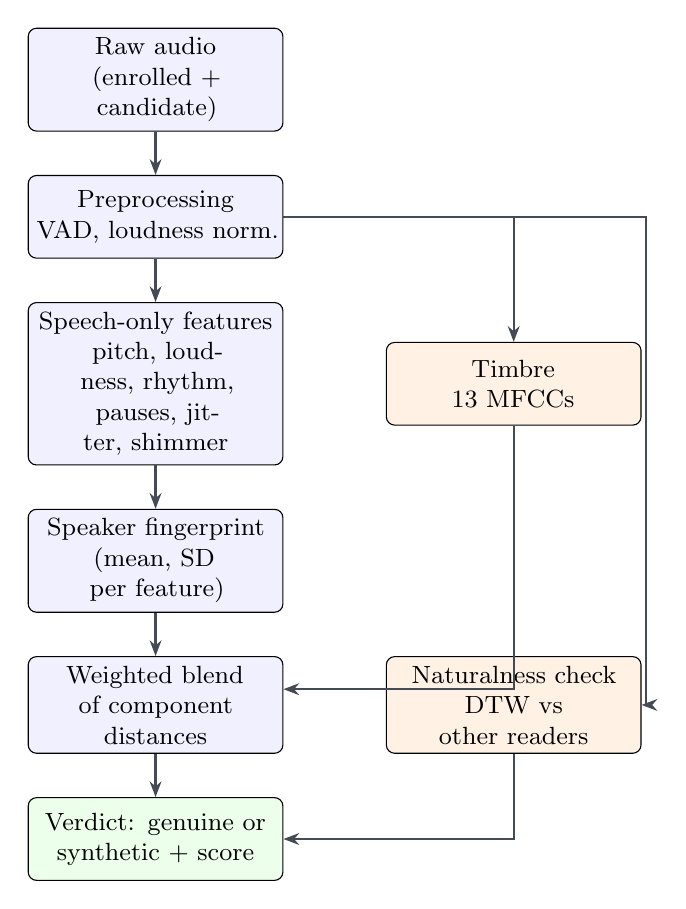
\begin{tikzpicture}[
  box/.style={draw, rounded corners=3pt, fill=blue!6, align=center, font=\small, minimum height=1.05cm, text width=3.0cm},
  alt/.style={box, fill=orange!10},
  res/.style={box, fill=green!8},
  arr/.style={-{Stealth[length=2mm]}, thick, ink2},
  node distance=0.55cm and 0.7cm]
\node[box] (in) {Raw audio\\(enrolled + candidate)};
\node[box, below=of in] (pre) {Preprocessing\\VAD, loudness norm.};
\node[box, below=of pre] (feat) {Speech-only features\\pitch, loudness, rhythm,\\pauses, jitter, shimmer};
\node[box, below=of feat] (fp) {Speaker fingerprint\\(mean, SD per feature)};
\node[box, below=of fp] (blend) {Weighted blend\\of component distances};
\node[alt, right=1.3cm of feat] (mfcc) {Timbre\\13 MFCCs};
\node[alt, right=1.3cm of blend] (nat) {Naturalness check\\DTW vs other readers};
\node[res, below=of blend] (dec) {Verdict: genuine or\\synthetic + score};
\draw[arr] (in) -- (pre); \draw[arr] (pre) -- (feat); \draw[arr] (feat) -- (fp); \draw[arr] (fp) -- (blend); \draw[arr] (blend) -- (dec);
\draw[arr] (pre.east) -| (mfcc.north); \draw[arr] (mfcc.south) |- ([yshift=2mm]blend.east);
\draw[arr] (pre.east) ++(0,0) -- ++(4.6,0) |- (nat.east);
\draw[arr] (nat.south) |- (dec.east);
\end{tikzpicture}
\caption{VoiceGuard pipeline. Prosody, voice quality, timbre and pitch level feed a weighted fingerprint score; the naturalness check runs alongside it on the same speech.}
\label{fig:pipeline}
\end{figure}

\subsection{Data Collection}
Three speakers (krishiv, mary and raghav) each read the same 30 prompt sentences on the same phone in the same room (AAC, 48\,kHz, mono, 3--8\,s per clip). Using identical text means differences between speakers reflect how they speak rather than what they say. Sentences s01--s20 form the \emph{enrollment} set; s21--s30 are \emph{held out} for testing and are the only text the cloners synthesize. Prompts include commas, lists and questions to give natural places to pause. Krishiv and raghav have Indian English accents and similar pitch (median about 132 and 125\,Hz); mary has an English accent (about 223\,Hz). Krishiv and mary read in a polished style and rarely pause; raghav pauses far more (4.7 internal pauses per clip).

An earlier pilot of 10 clips per speaker revealed four recordings filed under the wrong speaker, flagged independently by pitch, MFCCs and voice quality. The pilot was replaced by the matched-text set above.

\subsection{Preprocessing}
Audio is resampled to 16\,kHz mono and RMS-normalized to $-20$\,dBFS. Voice-activity detection (webrtcvad, 30\,ms frames) marks speech and silence; silence is kept as information, and internal pauses (at least 50\,ms, not touching the clip edges) become features. \textbf{All prosodic and voice-quality features are computed on detected speech only.} Section~\ref{sec:artifact} explains why this matters.

\subsection{Features}
Pitch is tracked with pYIN~\cite{pyin} (64\,ms frames, 16\,ms hop). Table~\ref{tab:features} lists the features, grouped into the four components the detector weights. Pitch-movement features are measured in semitones relative to the clip's own median, so they describe how pitch moves rather than how high the voice is; pitch level is a separate component measured against the claimed speaker's median.

\begin{table}[h]
\centering\small
\begin{tabularx}{\linewidth}{@{}l>{\raggedright\arraybackslash}Xl@{}}
\toprule
Component & Features (per clip) & Tool\\
\midrule
Prosody & pitch variability, range (p90--p10), slope, velocity, final rise/fall; loudness variability and slope; speaking rate (onsets per second of speech); nPVI; voiced fraction (\%V-like); VarcoV, VarcoUV; pause count, mean and variance & librosa, webrtcvad\\
Voice quality & local jitter, local shimmer & Parselmouth~\cite{parselmouth}\\
Timbre & 13 MFCCs, mean and SD (26 values) & librosa~\cite{librosa}\\
Pitch level & mean pitch in semitones vs.\ the speaker's median & pYIN\\
\bottomrule
\end{tabularx}
\caption{Features by detector component (15 prosodic, 2 voice-quality, 26 timbre, 1 pitch-level).}
\label{tab:features}
\end{table}

\subsection{Fingerprint and Detector}
For each component $c$, the speaker fingerprint is the per-feature mean $\mu$ and standard deviation $\sigma$ over the 20 enrollment clips, with a floor on $\sigma$ at each feature's measurement resolution (e.g.\ one 30\,ms VAD frame for pause durations). A candidate clip's distance on component $c$ is its root-mean-square $z$-score, with each $|z|$ clipped at 5:
\begin{equation}
d_c = \sqrt{\tfrac{1}{|c|}\textstyle\sum_{f\in c} z_f^2}, \qquad z_f = \frac{x_f-\mu_f}{\sigma_f}.
\end{equation}
The final score is a weighted average of component distances, with the non-prosodic components capped:
\begin{equation}
d = \frac{\sum_c w_c \min(d_c,\, \kappa_c)}{\sum_c w_c},
\end{equation}
with weights $w$ = 0.60 (prosody), 0.15 (voice quality), 0.15 (timbre) and 0.10 (pitch level), and caps $\kappa = 2$\,SD on all but prosody. Weights and caps were fixed by hand before evaluation; three speakers are too few to learn them without overfitting. Caps matter because a weight limits how much a component \emph{can} count, not how much it \emph{does}: without caps, pitch level (one feature, weight 0.10) jumped to 5\,SD for a different speaker and dominated the score. The accept threshold is the 90th percentile of leave-one-out distances of the enrollment clips, so about 10\% of genuine clips are rejected by design.

The proposal's primary model was a one-class SVM. A linear one-class SVM proved degenerate on standardized features: it separates data from the origin, and standardization centres the data on the origin, so on its own training clips its offset was about $10^{-8}$ and every decision value lay within $\pm0.001$. The distance detector above is the direct, interpretable form of the same one-class idea.

\subsection{Naturalness Check}
For a clip claiming to be speaker $X$ and reading prompt sentence $n$, we build frame-level contours of pitch (semitones vs.\ the clip's median) and loudness (dB vs.\ the clip's median) over its voiced speech, align them with dynamic time warping~\cite{dtw} to every \emph{other} enrolled speaker's reading of $n$, and average the distance. Each alignment yields a contour distance (mean frame difference along the path) and a timing distance (variation of local tempo along the path, with overall speed factored out). $X$'s own reading is never used, so genuine and cloned clips are scored the same way and no second recording of each sentence is needed. Each speaker's threshold is the 90th percentile of their naturalness distance on the enrollment sentences. This check asks ``is this read like a person reads it'', not ``is this speaker $X$''.

\subsection{Clone Generation and Accent Verification}
Clones were generated locally with two open-source zero-shot cloners, using only each speaker's enrollment audio (s01--s20) as the voice sample, to speak the held-out sentences s21--s30:
\begin{itemize}
\item \textbf{XTTS-v2}~\cite{xtts}: all 20 enrollment clips as reference. 30 clones; one (raghav, s26) was a 21\,s babbling failure and is excluded by the pipeline's 15\,s limit, leaving 29.
\item \textbf{F5-TTS}~\cite{f5tts}: one or two enrollment sentences (5.3--11.5\,s) with their exact transcript as reference. 30 clones.
\end{itemize}
Neither cloner exposes an accent control; accent comes from the reference audio. We verified it with a pretrained accent classifier (SpeechBrain CommonAccent ECAPA~\cite{commonaccent}, 16 English accents), reported in Section~\ref{sec:results}.

\subsection{Implementation}
Python with librosa, Parselmouth, webrtcvad, scikit-learn and NumPy; Coqui TTS and F5-TTS in separate environments; SpeechBrain for the accent check. A command-line tool (\texttt{cli.py enroll} / \texttt{cli.py score}) enrolls a speaker and scores a clip, and an interactive web front end (VoiceGuard Lab) visualizes every pipeline stage for each held-out clip.


% ---------------------------------------------------------------- 4
\section{Experimental Setup}
\label{sec:setup}
Each speaker is enrolled on their genuine sentences s01--s20. Testing uses only held-out sentences s21--s30: 30 genuine clips (10 per speaker), 30 F5-TTS clones and 29 XTTS-v2 clones of the same sentences, each scored against the claimed speaker's model. A second protocol, the \emph{impostor} task, scores each speaker's held-out clips against the other two speakers' models (60 impostor trials), measuring whether the fingerprint separates real people. We report ROC-AUC and equal error rate (EER), which do not depend on a threshold, and the share of clones rejected and genuine clips accepted at the deployed threshold.

Four systems are compared: the weighted blend (deployed), prosody only, pitch level plus timbre only (the cues a cloner is built to copy), and the naturalness check.

% ---------------------------------------------------------------- 5
\section{Results}
\label{sec:results}

\subsection{Accent Preservation}
Table~\ref{tab:accent} shows the accent classifier's top label per clip. XTTS-v2 Americanized all three speakers and placed their pitch about 3 semitones too low; F5-TTS kept krishiv's and raghav's Indian accents and mary's English accent. F5-TTS clones therefore sound like the speaker, not only like their voice.

\begin{table}[h]
\centering\small
\begin{tabular}{@{}llll@{}}
\toprule
Speaker & Genuine & XTTS-v2 clones & F5-TTS clones\\
\midrule
krishiv & Indian 30/30 & US 8/10, Canada 2/10 & Indian 10/10\\
mary & England 20/30, US 9/30 & US 8/10, England 2/10 & England 10/10\\
raghav & Indian 30/30 & US 7/9 & Indian 9/10, US 1/10\\
\bottomrule
\end{tabular}
\caption{Accent classifier (CommonAccent ECAPA) top label per clip.}
\label{tab:accent}
\end{table}

\subsection{Clone Detection}
Table~\ref{tab:clones} and Figure~\ref{fig:roc} summarize detection on held-out sentences. The weighted blend catches almost all XTTS-v2 clones and about three quarters of F5-TTS clones. Against the accent-preserving F5-TTS, prosody alone is the weakest of the fingerprint systems, and pitch level with timbre is the strongest.

\begin{table}[h]
\centering\small
\setlength{\tabcolsep}{5pt}
\begin{tabular}{@{}lccccccc@{}}
\toprule
 & \multicolumn{3}{c}{F5-TTS} & \multicolumn{3}{c}{XTTS-v2} & Genuine\\
\cmidrule(lr){2-4}\cmidrule(lr){5-7}
System & AUC & EER & rejected & AUC & EER & rejected & accepted\\
\midrule
Weighted blend (deployed) & 0.823 & 28.6\% & 73\% & 0.956 & 8.5\% & 97\% & 80\%\\
Prosody only & 0.685 & 38.6\% & 46\% & 0.872 & 20.3\% & 79\% & 80\%\\
Pitch level + timbre only & 0.880 & 19.3\% & 81\% & 0.990 & 6.8\% & 98\% & 77\%\\
Naturalness check & 0.671 & 35.0\% & 43\% & 0.661 & 40.7\% & 48\% & 87\%\\
\bottomrule
\end{tabular}
\caption{Clone detection on held-out sentences (30 genuine, 30 F5-TTS, 29 XTTS-v2 clips). ``Rejected'' and ``accepted'' are at the deployed threshold.}
\label{tab:clones}
\end{table}

\begin{figure}[h]
\centering
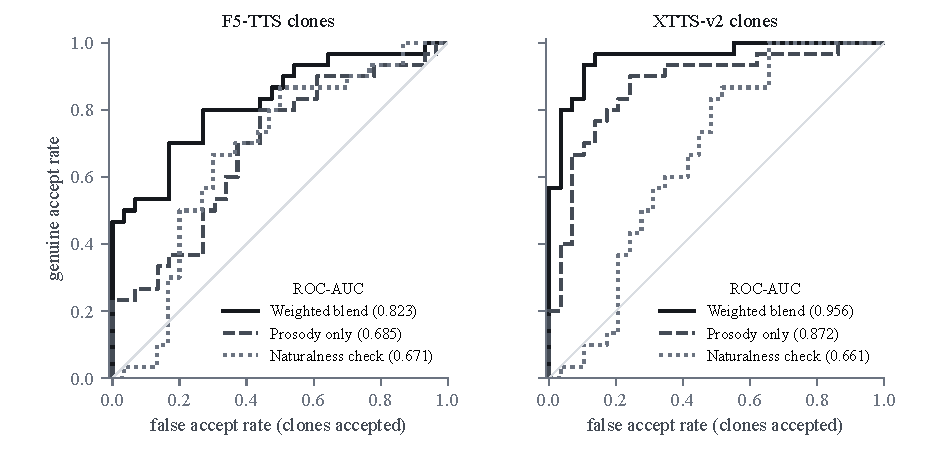
\includegraphics[width=\linewidth]{figures/fig-roc.pdf}
\caption{ROC curves on held-out clips, per cloner. Legend values are ROC-AUC.}
\label{fig:roc}
\end{figure}

Per speaker, the blend's ROC-AUC on F5-TTS clones is 0.87 (krishiv), 0.95 (mary) and 0.84 (raghav); on XTTS-v2 it is 0.99, 1.00 and 0.80. At the deployed threshold the blend rejects all of raghav's F5-TTS clones but only half of mary's: her clones rank well below her genuine clips (AUC 0.95) but fall inside her accept threshold. On the impostor task the blend reaches ROC-AUC 0.901 (prosody only 0.803), and prosody drives 63\% of the gap between genuine and impostor scores.

\subsection{What Gives Clones Away}
Figure~\ref{fig:tells} ranks every feature by how well it alone separates genuine clips from clones, and Figure~\ref{fig:contours} shows one sentence in all three versions.

\begin{figure}[h]
\centering
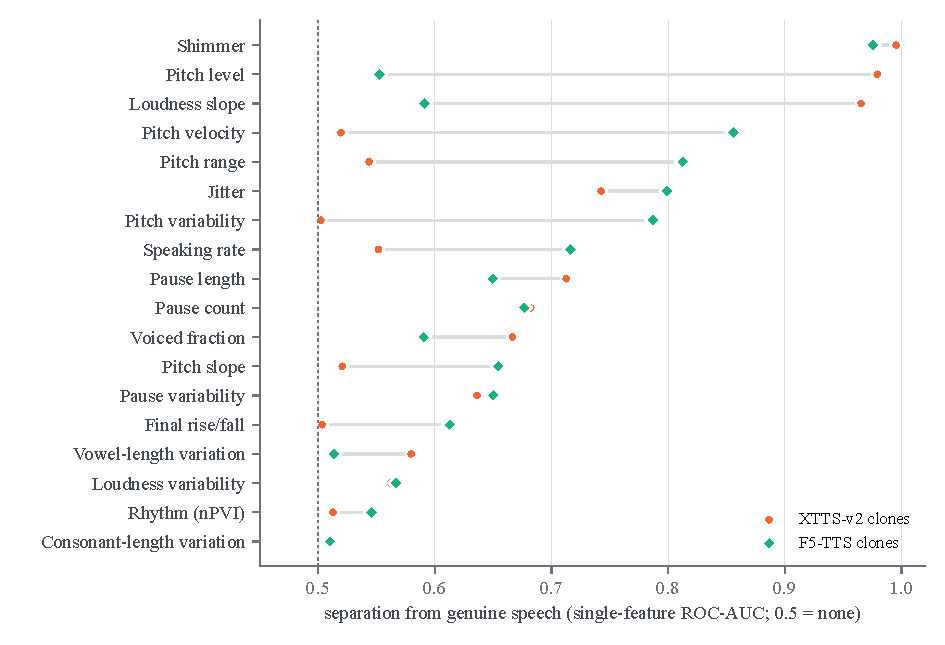
\includegraphics[width=0.92\linewidth]{figures/fig-tells.pdf}
\caption{Single-feature separation of genuine held-out clips from clones (ROC-AUC, each speaker standardized to their own genuine clips; 0.5 = no separation).}
\label{fig:tells}
\end{figure}

\begin{itemize}
\item \textbf{Too smooth (both cloners).} Shimmer, the cycle-to-cycle variation in loudness, is lower in clones and separates both cloners almost perfectly (0.995 XTTS-v2, 0.976 F5-TTS). It is the only tell common to both.
\item \textbf{Flat, slow intonation (F5-TTS).} Pitch moves more slowly (16.9 vs.\ 20.8 semitones per second, separation 0.86) over a narrower range (4.6 vs.\ 6.7 semitones, 0.81). XTTS-v2 reproduces both almost exactly (0.52 and 0.54).
\item \textbf{Fading out (XTTS-v2).} Loudness falls through each sentence (separation 0.97), and pitch sits about 3 semitones too low (0.98). F5-TTS shows neither.
\item \textbf{Pauses.} XTTS-v2 pauses about three times longer than the speakers. This is conspicuous for krishiv and mary, who rarely pause, but normal for raghav, which is why prosody alone misses many of his XTTS-v2 clones (0.57).
\end{itemize}

\begin{figure}[h]
\centering
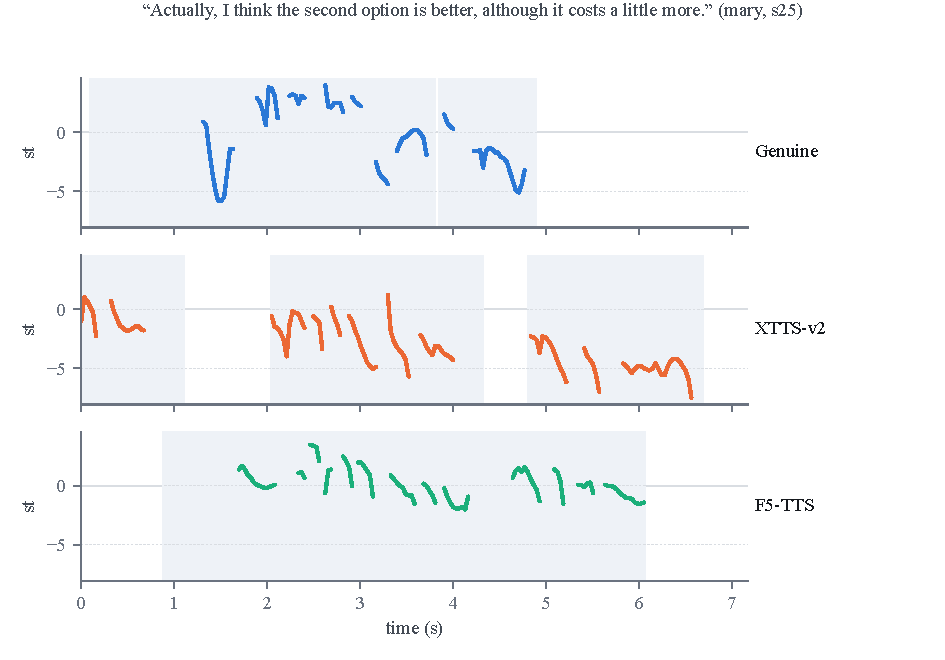
\includegraphics[width=0.92\linewidth]{figures/fig-contours.pdf}
\caption{Pitch contours (semitones vs.\ mary's median) of one held-out sentence: genuine, XTTS-v2 and F5-TTS. Shading marks detected speech. The F5-TTS clone's intonation is visibly flatter.}
\label{fig:contours}
\end{figure}

\subsection{Naturalness Check}
Once restricted to detected speech, the naturalness check separates clones only weakly (ROC-AUC 0.67 for both cloners; Figure~\ref{fig:naturalness}). Genuine readings sit about 1.7 from other people's readings of the same sentence, XTTS-v2 clones about 2.0, and F5-TTS clones between 1.7 and 2.0 depending on the speaker. With only two other readers per sentence, the human reference is too narrow to make this check decisive.

\begin{figure}[h]
\centering
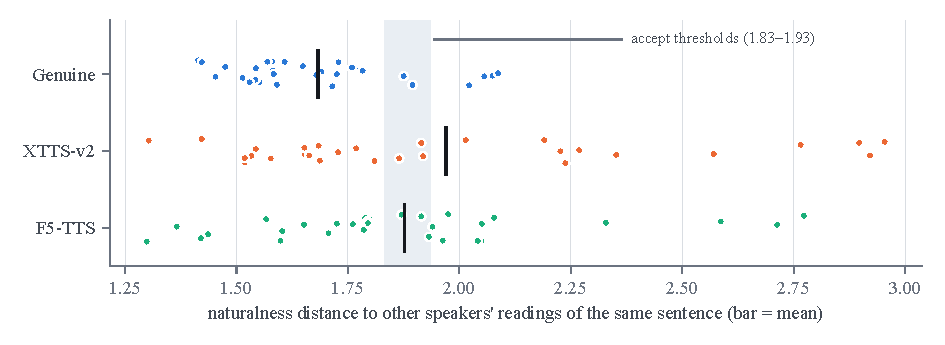
\includegraphics[width=\linewidth]{figures/fig-naturalness.pdf}
\caption{Naturalness distance on held-out clips, by source. The shaded band spans the three speakers' accept thresholds.}
\label{fig:naturalness}
\end{figure}

\subsection{A Measurement Artifact}
\label{sec:artifact}
An earlier version of the pipeline computed pitch, rhythm and voice-quality features over every voiced frame of a clip rather than only inside detected speech. 28 of 30 F5-TTS clones contain about 0.6\,s of low hum before speech begins (9 of 30 genuine clips have any, averaging 0.07\,s), which the pitch tracker reports as flat voiced pitch. That hum alone produced an apparent F5-TTS pitch slope of $+0.89$ semitones per second against $-1.30$ for genuine speech (separation 0.97), and inflated the naturalness check to ROC-AUC 0.964. Restricted to speech, the slope difference nearly disappears ($-0.85$ vs.\ $-1.30$, separation 0.65) and the naturalness check falls to 0.67. All results in this paper use the corrected, speech-only pipeline. The hum is itself detectable, but it is a synthesis artifact rather than prosody, and the next version of a cloner may not produce it.

% ---------------------------------------------------------------- 6
\section{Discussion}
\paragraph{Is the hypothesis supported?} Partly. Each cloner misses some of a speaker's prosodic habits (XTTS-v2 their loudness dynamics and pausing, F5-TTS their pitch movement), and a prosody-led detector catches 97\% and 73\% of their clones. But the habits each cloner misses are different, and against the cloner that preserves accent, prosody alone (ROC-AUC 0.685) is weaker than pitch level and timbre (0.880). Prosody is a useful, complementary signal, not yet a replacement for spectral cues.

\paragraph{Why prosody alone underperforms its best features.} Individual prosodic features separate F5-TTS clones well (pitch velocity 0.86, pitch range 0.81), yet the 15-feature prosody distance reaches only 0.685. The distance weights every feature equally, so a few informative features are diluted by many that carry little signal for a given cloner. Learning feature weights would help, but only if tested on a cloner the weights were not learned from; otherwise the detector learns one cloner's quirks.

\paragraph{Voice quality as a universal tell.} Shimmer separated both cloners almost perfectly. It reflects natural cycle-to-cycle irregularity of the voice, which both generators smooth away. In the deployed blend it carries only 15\% weight and a 2\,SD cap, chosen before evaluation; this is the clearest candidate for reweighting in future work.

\subsection{Deviations from the Proposal}
\label{sec:deviations}
\begin{itemize}
\item \textbf{Detector.} The proposed one-class SVM was degenerate on standardized features (Section 3.5) and was replaced by the distance-from-fingerprint detector, which implements the same one-class idea.
\item \textbf{Spectral baseline.} ECAPA-TDNN was replaced by an MFCC timbre component; the ``pitch level + timbre'' system plays the baseline's role.
\item \textbf{Learned sequence embedding, sequence classifiers.} Not built: three speakers are too few to train them.
\item \textbf{Data.} Public corpora (VoxCeleb, LibriSpeech, ASVspoof, WaveFake) were not used; all speech was self-recorded. RVC voice conversion was replaced by F5-TTS.
\item \textbf{Robustness and listening study.} Emotional-state robustness and the human listening study were not run.
\item \textbf{Tools.} webrtcvad replaced pyannote.audio, RMS normalization replaced EBU R128, and onset rate replaced forced-alignment speaking rate.
\end{itemize}

% ---------------------------------------------------------------- 7
\section{Limitations}
\begin{itemize}
\item \textbf{Small sample.} 30 genuine and 59 clone trials give wide uncertainty; one misclassified genuine clip moves the acceptance rate by over 3 percentage points.
\item \textbf{Two cloners.} The cloners fail in different ways, so a third may fail in yet another.
\item \textbf{Read speech.} Reading prompt sentences evens out prosody; conversational speech may separate speakers and clones differently.
\item \textbf{Same session, same device.} Genuine clips were recorded in one setting, so session-to-session variation is underrepresented.
\item \textbf{Hand-set weights.} Component weights and caps were fixed before evaluation rather than learned.
\end{itemize}

% ---------------------------------------------------------------- 8
\section{Conclusion and Future Work}
VoiceGuard shows that voice clones from two current open-source cloners leave measurable prosodic traces (loudness fade-out and long pauses in one, flattened and slowed intonation in the other) plus an over-smooth voice in both. A prosody-led detector built from 20 enrollment sentences per speaker catches 97\% of XTTS-v2 clones and 73\% of accent-preserving F5-TTS clones while accepting 80\% of genuine speech. Prosody is a real but partial signal: it complements spectral cues rather than replacing them, and which prosodic cue matters depends on the cloner. We also found that restricting every feature to detected speech is essential, because synthesis artifacts outside speech can masquerade as prosody.

Future work: learn component and feature weights across cloners and test on an unseen one; reweight voice quality; add speakers, spontaneous speech and multiple recording sessions; evaluate emotional-state robustness and run the planned listening study; and test against cloners explicitly trained to imitate a target's prosody.


\clearpage
\begin{thebibliography}{99}
\bibitem{dehak} N.~Dehak, P.~Dumouchel, and P.~Kenny, ``Modeling prosodic features with joint factor analysis for speaker verification,'' \emph{IEEE Transactions on Audio, Speech, and Language Processing}, vol.~15, no.~7, pp.~2095--2103, 2007.
\bibitem{prosodyid} Study on incorporating long-time-scale prosodic information (fundamental frequency and energy trajectory modelling) into speaker identification systems, evaluated on the NIST 2001 Speaker ID Extended Data Task using Switchboard-I conversational data.
\bibitem{survey} ``State-of-the-art in speaker recognition,'' survey covering short-term spectral and long-term prosodic feature classes in modern speaker-recognition systems, arXiv:2202.12705.
\bibitem{ecapa} B.~Desplanques, J.~Thienpondt, and K.~Demuynck, ``ECAPA-TDNN: Emphasized Channel Attention, Propagation and Aggregation in TDNN Based Speaker Verification,'' in \emph{Proc. Interspeech}, 2020.
\bibitem{asvspoof} ASVspoof Consortium, ``ASVspoof: Automatic Speaker Verification Spoofing and Countermeasures Challenge Series,'' benchmark datasets and evaluation protocols for synthetic and replay speech detection.
\bibitem{wavefake} J.~Frank and L.~Sch\"onherr, ``WaveFake: A Data Set to Facilitate Audio Deepfake Detection,'' in \emph{NeurIPS Datasets and Benchmarks Track}, 2021.
\bibitem{forensic} Overview of forensic speaker verification methodology and known sources of intra-speaker variability (age, health, emotional state) affecting voice-biometric reliability.
\bibitem{pyin} M.~Mauch and S.~Dixon, ``pYIN: A fundamental frequency estimator using probabilistic threshold distributions,'' in \emph{Proc. IEEE ICASSP}, 2014, pp.~659--663.
\bibitem{grabe} E.~Grabe and E.~L.~Low, ``Durational variability in speech and the rhythm class hypothesis,'' in \emph{Papers in Laboratory Phonology 7}, 2002, pp.~515--546.
\bibitem{ramus} F.~Ramus, M.~Nespor, and J.~Mehler, ``Correlates of linguistic rhythm in the speech signal,'' \emph{Cognition}, vol.~73, no.~3, pp.~265--292, 1999.
\bibitem{dellwo} V.~Dellwo, ``Rhythm and speech rate: A variation coefficient for $\Delta$C,'' in \emph{Language and Language-Processing}, 2006, pp.~231--241.
\bibitem{dtw} H.~Sakoe and S.~Chiba, ``Dynamic programming algorithm optimization for spoken word recognition,'' \emph{IEEE Transactions on Acoustics, Speech, and Signal Processing}, vol.~26, no.~1, pp.~43--49, 1978.
\bibitem{parselmouth} Y.~Jadoul, B.~Thompson, and B.~de~Boer, ``Introducing Parselmouth: A Python interface to Praat,'' \emph{Journal of Phonetics}, vol.~71, pp.~1--15, 2018.
\bibitem{librosa} B.~McFee \emph{et al.}, ``librosa: Audio and music signal analysis in Python,'' in \emph{Proc. Python in Science Conference}, 2015.
\bibitem{xtts} E.~Casanova \emph{et al.}, ``XTTS: a Massively Multilingual Zero-Shot Text-to-Speech Model,'' in \emph{Proc. Interspeech}, 2024.
\bibitem{f5tts} Y.~Chen \emph{et al.}, ``F5-TTS: A Fairytaler that Fakes Fluent and Faithful Speech with Flow Matching,'' arXiv:2410.06885, 2024.
\bibitem{commonaccent} J.~Zuluaga-Gomez \emph{et al.}, ``CommonAccent: Exploring Large Acoustic Pretrained Models for Accent Classification Based on Common Voice,'' in \emph{Proc. Interspeech}, 2023.
\end{thebibliography}


\clearpage
\appendix
\section{Reproducibility}
All numbers in this paper are produced by the project repository's scripts:
\begin{itemize}
\item \texttt{python src/features.py}, \texttt{python src/spectral\_features.py}: features for all clips.
\item \texttt{python cli.py enroll <speaker> <s01--s20 clips>}: enrollment.
\item \texttt{python cli.py score <speaker> <clip> [-{}-sentence N]}: scoring.
\item \texttt{python src/impostor\_eval.py}: impostor, clone and ablation tables.
\item \texttt{python src/contour.py}: naturalness calibration and evaluation.
\item \texttt{src/generate\_clones.py} (XTTS-v2) and \texttt{src/generate\_clones\_f5.py} (F5-TTS): clone generation; \texttt{src/accent\_check.py}: accent verification.
\item \texttt{python src/export\_viz.py}, \texttt{python src/make\_figures.py}: VoiceGuard Lab data and the figures.
\end{itemize}

\end{document}
